\vspace{1cm}
\fancyhead[C]{\normalsize\textbf{$\qquad$ Teil I: Offene Aufgaben}}
\renewcommand{\labelenumi}{\theenumi.}
\section*{Aufgabe 1 (26 Punkte)}
\vspace{0.4cm}
\subsection*{\aufgabe{a1}{4}}
Gegeben ist die Funktion 
\begin{align*}
f  \ : \ D_f \to \mathbb{R},
\
x \mapsto \ln(\sqrt{x-2} - 4 ) + \ln(\sqrt{x-2} + 4).
\end{align*}
Ermitteln Sie den Definitionsbereich $ D_f $ und den Wertebereich $ W_f $ von $ f$.\\
\\
\textit{Hinweis:} Vereinfachen Sie zunächst die Logarithmusterme.
\\
\\
\textbf{Lösung:}
\begin{mdframed}
\underline{\textbf{Vorgehensweise:}}
\renewcommand{\labelenumi}{\theenumi.}
\begin{enumerate}
\item Forme den Ausdruck mithilfe der Logarithmusgesetze um.
\item Bestimme den Definitionsbereich $ D_f $.
\item Bestimme den Wertebereich $ W_f $.
\end{enumerate}
\end{mdframed}
\underline{1. Forme den Ausdruck mithilfe der Logarithmusgesetze um}\\
Wir benötigen das Logarithmusgesetz
\begin{align*}
\ln(a) + \ln(b) = \ln(a \cdot b)
\end{align*}
und die dritte binomische Formel
\begin{align*}
(a-b)(a+b) = a^2 - b^2.
\end{align*}
Damit erhalten wir mit 
\begin{align*}
f(x) = \ln(\sqrt{x-2} - 4 ) + \ln(\sqrt{x-2} + 4)
= \ln((\sqrt{x-2}-4) \cdot (\sqrt{x-2} +4))
= \ln(x-2 - 16) = \ln (x- 18)
\end{align*}
einen vereinfachten Ausdruck.
\\
\\
\underline{2. Bestimme den Definitionsbereich $ D_f $}\\
Der Logarithmus $ \ln(x) $ ist definiert, falls der Ausdruck im Logarithmus größer null ist.
Also erkennen  wir an unserem vereinfachten Ausdruck, dass die Funktion definiert ist, falls
\begin{align*}
x - 18 > 0 \ \Leftrightarrow \ x > 18
\end{align*}
gilt. Damit ist der Definitionsbereich $ D_f = (18,\infty) $.
\\
\\
\underline{3. Bestimme den Wertebereich $ W_f $}\\
Wir erinnern uns, dass der Logarithmus die Umkehrfunktion der Exponentialfunktion ist.
Der Definitionsbereich der Exponentialfunktion ist $ \mathbb{R} $. Dieser entspricht dem Wertebereich des $ \ln $, da beide Funktionen zueinander Umkehrfunktionen sind.
Der Wertebereich von 
\begin{align*}
x - 18 
\end{align*}
ist $ (0, \infty) $ für $ x > 18 $. Dementsprechend verwenden wir den kompletten Definitionsbereich der $ \ln $ Funktion.
Damit gilt $ W_f = \mathbb{R} $.

\newpage

\subsection*{\aufgabe{a2}{3}}
Gegeben ist die Funktion 
\begin{align*}
f  \ : \ D_f \to \mathbb{R},
\
x \mapsto \ln(\sqrt{x-2} - 4 ) + \ln(\sqrt{x-2} + 4).
\end{align*}
Ist die Funktion $ f  $ auf ihrem Definitionsgebiet streng konkav (Beweis)?
\\
\\
\textbf{Lösung:}
\begin{mdframed}
\underline{\textbf{Vorgehensweise:}}
\renewcommand{\labelenumi}{\theenumi.}
\begin{enumerate}
\item Definiere die Bedingung für Konkavität.
\item Berechne die erste und zweite Ableitung und löse die Aufgabe.
\end{enumerate}
\end{mdframed}

\underline{1. Definiere die Bedingung für Konkavität}\\
Eine Funktion $ f \: \ D_f \to \mathbb{R} $ heisst streng konkav, falls
\begin{align*}
f^{\prime \prime}(x) < 0
\end{align*}
für alle $ x \in D_f $ gilt. Wir müssen also die zweite Ableitung bestimmen.
\\
\\
\underline{2. Berechne die erste und zweite Ableitung und löse die Aufgabe}\\
Wir verwenden 
\begin{align*}
f(x) = \ln(x - 18)
\end{align*}
aus der ersten Aufgabe.
Damit erhalten wir:
\begin{align*}
f^\prime(x) &=  \frac{1}{x -18} = (x-18)^{-1}  \\
f^{\prime \prime}(x) &= -1 \cdot (x-18)^{-2} = \frac{-1}{(x-18)^2}
\end{align*}
Wegen $ (x-18)^2  > 0 $ für $ x > 18 $ gilt
\begin{align*}
f^{\prime \prime}(x) < 0 
\end{align*}
für $ x \in D_f = (18,\infty) $.
Damit ist $ f $ streng konkav.
\newpage
\subsection*{\aufgabe{a3}{3}}
Gegeben ist die Funktion 
\begin{align*}
f  \ : \ D_f \to \mathbb{R},
\
x \mapsto \ln(\sqrt{x-2} - 4 ) + \ln(\sqrt{x-2} + 4).
\end{align*}
Ermitteln Sie die Umkehrfunktion $ f^{-1} $ von $ f $.
\\
\\
\textbf{Lösung:}
\begin{mdframed}
\underline{\textbf{Vorgehensweise:}}
\begin{enumerate}
\item Bestimme die Umkehrfunktion.
\end{enumerate}
\end{mdframed}

\underline{1. Bestimme die Umkehrfunktion}\\
Um die Umkehrfunktion zu bestimmen, müssen wir
\begin{align*}
y = \ln(x-18)
\end{align*}
nach $ x $ umformen. 
Wichtig ist hier, dass die Exponentialfunktion die Umkehrfunktion der Logarithmusfunktion ist, d.h. es gilt:
\begin{align*}
x = e^ {\ln(x)} = \ln(e^x).
\end{align*}
Es gilt
\begin{align*}
y = \ln(x - 18)
\ 
\Leftrightarrow
\
e^y = x - 18
\
\Leftrightarrow
\
x = e^y + 18
\end{align*}
und durch Vertauschen von $ x  $ und $ y $ erhalten wir
\begin{align*}
f^{-1}(x ) = e^x + 18
\end{align*}
als Umkehrfunktion.

\newpage
\subsection*{\aufgabe{b}{6}}
Um seine Geschäftsidee zu finanzieren, nimmt ein Start-up einen Kredit in Höhe von
$ 1' 0 00 '0 0 0 $ CHF auf. Die Bank stimmt einem niedrigeren jährlichen Zinssatz von $ 0.5\% $
während der ersten 5 Jahre zu, in denen das Start-up am Ende jeden Jahres $ 10'000 $ CHF
zurückzahlen muss. Danach steigt der Zinssatz auf $ 2 \% $ p.a. und es werden konstante
Zahlungen in Höhe von $ C^I $ CHF vereinbart, die wieder am Ende jeden Jahres fällig sind.
Der Plan sieht vor, dass der Kredit in 15 Jahren zurückgezahlt ist.
\\
\\
Wie hoch müssen die jährlichen Zahlungen $ C^I $ sein, sodass der Plan des Start-ups umsetzbar ist?
\\
\\
\textbf{Lösung:}
\begin{mdframed}
\underline{\textbf{Vorgehensweise:}}
\begin{enumerate}
\item Bestimme den Endwert für die Jahre $ 1 $-$ 5 $.
\item Bestimme den Endwert für die Jahre $ 6$-$ 15 $.
\item Bestimme die jährlichen Zahlungen $ C^I $.
\end{enumerate}
\end{mdframed}

\underline{1. Bestimme den Endwert für die Jahre $ 1 $-$ 5 $}\\
Da am Ende jeden Jahres 10'000 CHF zurückgezahlt werden, erhalten wir eine 5-jährige nachschüssige Rente. Durch den jährlichen Zinssatz von $0.5 \%$ ist deren Endwert durch
\begin{align*}
A_5 = 10'000 \cdot \frac{(1+ 0.5 \%)^5 -1 }{0.5 \%} \approx 50'502.50 \ \text{CHF}
\end{align*}
gegeben.
\\
\\
\underline{2. Bestimme den Endwert für die Jahre $ 6 $-$ 15 $}\\
Durch die Zahlungen $C^I$ CHF ist für die darauffolgenden 10 Jahre eine nachschüssige 10-jährige Rente gegeben. Aufgrund des Zinssatzes von $2 \%$ ist deren Endwert durch
\begin{align*}
A_{10} = C^I \cdot \frac{(1+ 2.0 \%)^{10} -1}{2.0 \%}
\end{align*}
gegeben.
\\
\\
\newpage
\underline{3. Bestimme die jährlichen Zahlungen $ C^I $}\\
Um $ C^I $ zu bestimmen, muss der Barwert $ 1'000'000 $ und der Barwert der Renten identisch sein. Dies führt auf die Gleichung:
\begin{align*}
1'000'000 = 
\frac{A_5}{(1+ 0.5 \%)^5} +
\frac{A_{10}}{(1+ 0.5 \%)^5(1+2.0 \%)^{10}}
\end{align*}
Unser Ziel ist nun nach der in $A_{10}$ steckenden Konstante umzuformen. Hierfür betrachten wir
\begin{align*}
1'000'000
&= \frac{1}{(1+ 0.5 \%)^5} \cdot 
10'000 \cdot \frac{(1+ 0.5 \%)^5 -1 }{0.5 \%}
+ 
\frac{1}{(1+ 0.5 \%)^5 (1 + 2 \%)^{10}} \cdot 
C^I \cdot \frac{(1+ 2.0 \%)^{10} -1}{2.0 \%}\\
&\Leftrightarrow
1'000'000 (1+ 0.5 \%)^5
=
10'000 \cdot \frac{(1+ 0.5 \%)^5 -1 }{0.5 \%}
+
\frac{1}{(1 + 2 \%)^{10}} \cdot C^I \cdot \frac{(1+ 2.0 \%)^{10} -1}{2.0 \%}\\
&\Leftrightarrow
1'000'000 (1+ 0.5 \%)^5 - 10'000 \cdot \frac{(1+ 0.5 \%)^5 -1 }{0.5 \%} 
=
\frac{1}{(1 + 2 \%)^{10}} \cdot C^I \cdot \frac{(1+ 2.0 \%)^{10} -1}{2.0 \%}\\
&\Leftrightarrow 
(1 + 2 \%)^{10} \left(  1'000'000 (1+ 0.5 \%)^5 - 10'000 \cdot \frac{(1+ 0.5 \%)^5 -1 }{0.5 \%} \right)
=
C^I \cdot \frac{(1+ 2.0 \%)^{10} -1}{2.0 \%}\\
&\Leftrightarrow
\frac{2.0 \%}{(1+ 2.0 \%)^{10} -1}(1 + 2 \%)^{10} \left(  1'000'000 (1+ 0.5 \%)^5 - 10'000 \cdot \frac{(1+ 0.5 \%)^5 -1 }{0.5 \%} \right) = C^I
\end{align*} 
und erhalten gerundet die jährlichen Zahlungen
\begin{align*}
C^I \approx 108'515.40 \ \text{CHF}.
\end{align*}

\newpage

\subsection*{\aufgabe{c}{4}}
Berechnen Sie 
\begin{align*}
\lim \limits_{x \to 0} \frac{2}{x^4} e^{- \frac{1}{x^2}}.
\end{align*}
\\
\\
\textbf{Lösung:}
\begin{mdframed}
	\underline{\textbf{Vorgehensweise:}}
	\begin{enumerate}
		\item Bringe den Ausdruck in eine Form, um de l'H\^{o}pital anzuwenden.
		\item Alternativer Lösungsweg.
	\end{enumerate}
\end{mdframed}

\underline{1. Bringe den Ausdruck in eine Form, um de l'H\^{o}pital anzuwenden und bestimme den Grenzwert}\\
Wir substituieren 
\begin{align*}
y = \frac{1}{x^2}
\end{align*}
und erhalten 
\begin{align*}
\frac{2}{x^4} e^{- \frac{1}{x^2}}
=2 y^2 \cdot e^{-y}
= 2 \frac{y^2}{e^{y}}.
\end{align*}
Wegen 
\begin{align*}
\lim \limits_{x \to 0} \frac{1}{x^2} = \infty
\end{align*}
gilt $ y \to \infty $.
Damit erhalten wir mithilfe der Regel von de l'H\^{o}pital:
\begin{align*}
\lim \limits_{x \to 0} \frac{2}{x^4} e^{- \frac{1}{x^2}}
=
\lim \limits_{y \to \infty} 2 \frac{y^2}{e^{y}}
=
\lim \limits_{y \to \infty} \frac{4y}{e^{y}}
=
\lim \limits_{y \to \infty}  \frac{4}{e^{y}} = 0
\end{align*}
\\
\\
\underline{2. Alternativer Lösungsweg}\\
Es gilt
\begin{align*}
\frac{2}{x^2} e^{-\frac{1}{x^2}}
=
\frac{2 \cdot \frac{1}{x^2}}{e^{\frac{1}{x^2}}}
\end{align*}
und wegen 
\begin{align*}
\lim \limits_{x \to 0 } \frac{1}{x^2} = \infty, \quad
\lim \limits_{x \to 0 } e^{\frac{1}{x^2}} = \infty
\end{align*}
können wir die Regel von l'H\^{o}pital anwenden.
Es gelten
\begin{align*}
\frac{\mathrm{d}}{\mathrm{d} x} \frac{1}{x^2}
&=
\frac{\mathrm{d}}{\mathrm{d} x} x^{-2} 
=
-2 x^{-3} = \frac{-2}{x^3}\\
\frac{\mathrm{d}}{\mathrm{d} x} e^{\frac{1}{x^2}}
&=
\frac{-2}{x^3} e^{\frac{1}{x^2}} 
\end{align*}
und durch die Regel von l'H\^{o}pital erhalten wir
\begin{align*}
\lim \limits_{x \to 0 } \frac{2 \cdot \frac{1}{x^2}}{e^{\frac{1}{x^2}}}
=
\lim \limits_{x \to 0 } \frac{2 \frac{-2}{x^3}}{\frac{-2}{x^3} e^{\frac{1}{x^2}}}
= 
\lim \limits_{x \to 0} \frac{2}{e^{\frac{1}{x^2}}} = 0
\end{align*}
als Grenzwert.\\
\\

\newpage
\subsection*{\aufgabe{d}{6}}
Eine professionelle Langstreckenläuferin läuft in der ersten Stunde 20 Kilometer. Danach nimmt ihre Leistung in jeder weiteren Stunde des Laufens um einen Faktor $ a \in (0,1] $ ab, dass heisst beispielsweise in der zweiten Stunde läuft sie noch $ 20 \cdot (1-a) $ Kilometer.
Für welche Werte $ a \in (0,1] $ und $ b \geq 20  $ wird die Läuferin einen Wettkampf der Länge von $ b  $ Kilometern bewältigen können, gegeben dass sie beliebig lange laufen kann?
\\
\\
Stellen Sie die Lösungsmenge graphisch (in einem (a,b)-System) dar.
\\
\\
\textbf{Lösung:}
\begin{mdframed}
	\underline{\textbf{Vorgehensweise:}}
	\begin{enumerate}
		\item Stelle die in der Stunde gelaufene Strecke mithilfe einer geometrischen Folge dar.
		
		\item
		Verwende die geometrische Reihe, um die Lösungsmenge graphisch darzustellen.
	\end{enumerate}
\end{mdframed}

\underline{1. Stelle die in der Stunde gelaufene Strecke mithilfe einer geometrischen Folge dar}\\
In der ersten Stunden wird $a_1 = 20$ gelaufen. Aufgrund der natürlichen Erschöpfung erhalten wir in der zweiten Stunde
$a_2 = a_1 (1 - a)$. Allgemein erhalten wir den den rekursiven Zusammenhang (d.h. das nachfolgende Folgenglied wird aus dem vorherigen Folgenglied berechnet)
\begin{align*}
a_1 &= 20\\
a_n &= a_{n-1} (1-a), \quad n = 2 , 3,...
\end{align*}
Aus dem rekursiven Zusammenhang erhalten wir mit
\begin{align*}
a_n = a_1 (1-a)^{n-1}
\end{align*}
eine explizite Formel für das $ n $-te Folgenglied.
\\
\\
\underline{2. Verwende die geometrische Reihe, um die Lösungsmenge graphisch darzustellen}\\
Unsere Folge liefert uns die in $ n $-ten Stunde gelaufene Strecke. Die Läuferin kann beliebig lange laufen, daher ist die gelaufene Strecke durch
\begin{align*}
\sum \limits_{n = 1}^\infty a_n 
=
\sum \limits_{n=1}^\infty a_1 (1-a)^{n-1}
= a_1 \sum \limits_{n=1}^\infty  (1-a)^{n-1}
= a_1 \sum \limits_{n=0}^\infty  (1-a)^{n}
%= a_1 \frac{1}{1 - (1-a)} 
%= \frac{a_1}{a} = \frac{20}{a}
\end{align*}
gegeben. Eine Summe der Form $ \sum_{n=0}^\infty q^n $
bezeichnet man als geometrische Reihe. Diese besitzt den den Grenzwert
\begin{align*}
\sum \limits_{n=0}^\infty q^n = \frac{1}{1-q},
\end{align*}
falls $ |q| < 1 $ erfüllt ist. In unserem Fall gilt
\begin{align*}
a_1 \sum \limits_{n=0}^\infty  (1-a)^{n} = a_1 \cdot \frac{1}{1-(1-a)} = \frac{a_1}{a} = \frac{20}{a},
\end{align*}
da $ | 1 -a | < 1 $ für $ a \in (0,1] $ erfüllt ist.
Da die Läuferin mindestens $ b \geq 20  $ Kilometer laufen muss, sollte nun 
\begin{align*}
\frac{20}{a} \geq b 
\end{align*} 
erfüllt sein. Wir erhalten also die Lösungsmenge
\begin{align*}
\mathcal{L}
:= \left\{ (a,b ) \in (0,1] \times [20,\infty) \ : \ b \leq \frac{20}{a}  \right\}
\end{align*}
und die zugehörige Skizze:
\begin{center}
	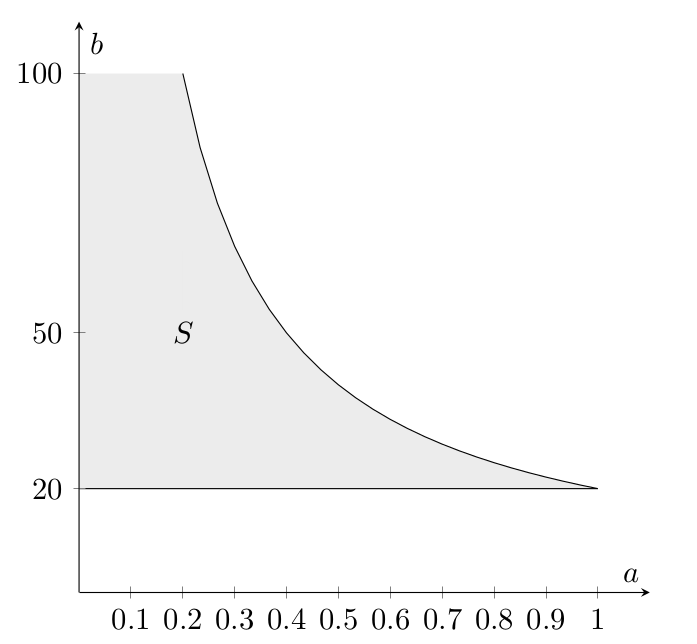
\includegraphics[width=0.5\textwidth]{pictures/auf1_d.png}
\end{center}

\newpage